
\documentclass[si.tex]{subfiles}

\begin{document}


\begin{comment}
python3 RunSynthetic_FreePrior_CosineLoss_OnSim_VIZ_OnlyModel_OtherNoiseLevels_WithGroundTruthPrior.py 2 0 10.0 180 SimulateSynthetic_Parameterized_OtherNoiseLevels_Grid_VarySize.py_180_2_2_N40000_UNIFORM_STEEPPERIODIC.txt
python3 RunSynthetic_FreePrior_CosineLoss_OnSim_VIZ_OnlyModel_OtherNoiseLevels_WithGroundTruthPrior.py 2 0 10.0 180 SimulateSynthetic_Parameterized_OtherNoiseLevels_Grid_VarySize.py_180_2_2_N40000_STEEPPERIODIC_STEEPPERIODIC.txt
python3 RunSynthetic_FreePrior_CosineLoss_OnSim_VIZ_OnlyModel_OtherNoiseLevels_WithGroundTruthPrior.py 2 0 10.0 180 SimulateSynthetic_Parameterized_OtherNoiseLevels_Grid_VarySize.py_180_2_2_N40000_STEEPPERIODIC_UNIFORM.txt
python3 RunSynthetic_FreePrior_CosineLoss_OnSim_VIZ_OnlyModel_OtherNoiseLevels_WithGroundTruthPrior.py 2 0 10.0 180 SimulateSynthetic_Parameterized_OtherNoiseLevels_Grid_VarySize.py_180_2_2_N40000_STEEPSHIFTED_STEEPPERIODIC.txt

python3 RunSynthetic_FreePrior_CosineLoss_OnSim_VIZ_OnlyModel_OtherNoiseLevels_WithGroundTruthPrior.py 2 0 10.0 180 SimulateSynthetic_Parameterized_OtherNoiseLevels_Grid_VarySize.py_180_2_5_N40000_UNIFORM_STEEPPERIODIC.txt
python3 RunSynthetic_FreePrior_CosineLoss_OnSim_VIZ_OnlyModel_OtherNoiseLevels_WithGroundTruthPrior.py 2 0 10.0 180 SimulateSynthetic_Parameterized_OtherNoiseLevels_Grid_VarySize.py_180_2_5_N40000_STEEPPERIODIC_STEEPPERIODIC.txt
python3 RunSynthetic_FreePrior_CosineLoss_OnSim_VIZ_OnlyModel_OtherNoiseLevels_WithGroundTruthPrior.py 2 0 10.0 180 SimulateSynthetic_Parameterized_OtherNoiseLevels_Grid_VarySize.py_180_2_5_N40000_STEEPPERIODIC_UNIFORM.txt
python3 RunSynthetic_FreePrior_CosineLoss_OnSim_VIZ_OnlyModel_OtherNoiseLevels_WithGroundTruthPrior.py 2 0 10.0 180 SimulateSynthetic_Parameterized_OtherNoiseLevels_Grid_VarySize.py_180_2_5_N40000_STEEPSHIFTED_STEEPPERIODIC.txt

python3 RunSynthetic_FreePrior_CosineLoss_OnSim_VIZ_OnlyModel_OtherNoiseLevels_WithGroundTruthPrior.py 2 0 10.0 180 SimulateSynthetic_Parameterized_OtherNoiseLevels_Grid_VarySize.py_180_2_2345_N40000_UNIFORM_STEEPPERIODIC.txt
python3 RunSynthetic_FreePrior_CosineLoss_OnSim_VIZ_OnlyModel_OtherNoiseLevels_WithGroundTruthPrior.py 2 0 10.0 180 SimulateSynthetic_Parameterized_OtherNoiseLevels_Grid_VarySize.py_180_2_2345_N40000_STEEPPERIODIC_STEEPPERIODIC.txt
python3 RunSynthetic_FreePrior_CosineLoss_OnSim_VIZ_OnlyModel_OtherNoiseLevels_WithGroundTruthPrior.py 2 0 10.0 180 SimulateSynthetic_Parameterized_OtherNoiseLevels_Grid_VarySize.py_180_2_2345_N40000_STEEPPERIODIC_UNIFORM.txt
python3 RunSynthetic_FreePrior_CosineLoss_OnSim_VIZ_OnlyModel_OtherNoiseLevels_WithGroundTruthPrior.py 2 0 10.0 180 SimulateSynthetic_Parameterized_OtherNoiseLevels_Grid_VarySize.py_180_2_2345_N40000_STEEPSHIFTED_STEEPPERIODIC.txt

\end{comment}



\begin{figure}
\centering

\begin{tikzpicture}[every node/.style={inner sep=0, anchor=north west}]

  % ========================
  % Only 1 Level (High Noise)
  % ========================
  \node[anchor=center,font=\bfseries] (t1) at (0.45\textwidth, 0.5) {Only 1 Level (High Noise)};

  % Row 1: first 4 PDFs (two “full‐model” + two “relativeLF”)
  \node (h1a) at (0, -0) {%
    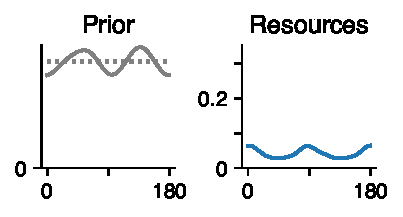
\includegraphics[width=0.3\textwidth]{figures/RunSynthetic_FreePrior_CosineLoss_OnSim_VIZ_OnlyModel_OtherNoiseLevels_WithGroundTruthPrior.py_SimulateSynthetic_Parameterized_OtherNoiseLevels_Grid_VarySize.py_180_2_2_N40000_UNIFORM_STEEPPERIODIC.txt_2_0_10.0_180.pdf}%
  };
  \node (h1b) at (0.3\textwidth, -0) {%
    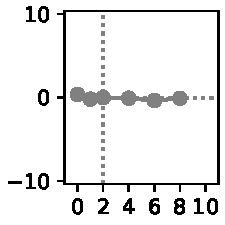
\includegraphics[width=0.14\textwidth]{figures/evaluateCrossValidationResults_Synthetic_Gardelle_NonF.py_SimulateSynthetic_Parameterized_OtherNoiseLevels_Grid_VarySize.py_180_2_2_N40000_UNIFORM_STEEPPERIODIC.txt_RelativeLF.pdf}%
  };
  \node (h1c) at (0.5\textwidth, -0) {%
    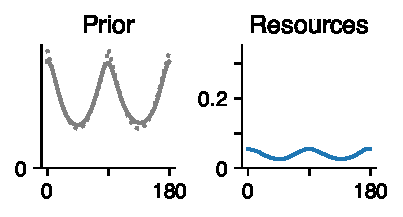
\includegraphics[width=0.3\textwidth]{figures/RunSynthetic_FreePrior_CosineLoss_OnSim_VIZ_OnlyModel_OtherNoiseLevels_WithGroundTruthPrior.py_SimulateSynthetic_Parameterized_OtherNoiseLevels_Grid_VarySize.py_180_2_2_N40000_STEEPPERIODIC_STEEPPERIODIC.txt_2_0_10.0_180.pdf}%
  };
  \node (h1d) at (0.8\textwidth, -0) {%
    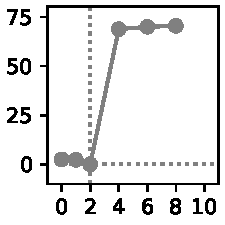
\includegraphics[width=0.14\textwidth]{figures/evaluateCrossValidationResults_Synthetic_Gardelle_NonF.py_SimulateSynthetic_Parameterized_OtherNoiseLevels_Grid_VarySize.py_180_2_2_N40000_STEEPPERIODIC_STEEPPERIODIC.txt_RelativeLF.pdf}%
  };

  % Row 2: next 4 PDFs
  \node (h2a) at (0, -2.5) {%
    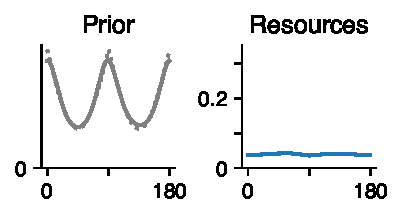
\includegraphics[width=0.3\textwidth]{figures/RunSynthetic_FreePrior_CosineLoss_OnSim_VIZ_OnlyModel_OtherNoiseLevels_WithGroundTruthPrior.py_SimulateSynthetic_Parameterized_OtherNoiseLevels_Grid_VarySize.py_180_2_2_N40000_STEEPPERIODIC_UNIFORM.txt_2_0_10.0_180.pdf}%
  };
  \node (h2b) at (0.3\textwidth, -2.5) {%
    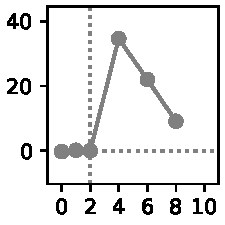
\includegraphics[width=0.14\textwidth]{figures/evaluateCrossValidationResults_Synthetic_Gardelle_NonF.py_SimulateSynthetic_Parameterized_OtherNoiseLevels_Grid_VarySize.py_180_2_2_N40000_STEEPPERIODIC_UNIFORM.txt_RelativeLF.pdf}%
  };
  \node (h2c) at (0.5\textwidth, -2.5) {%
    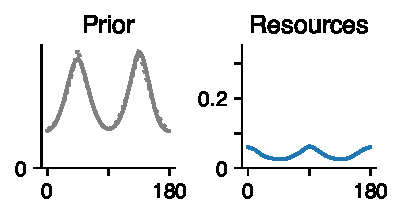
\includegraphics[width=0.3\textwidth]{figures/RunSynthetic_FreePrior_CosineLoss_OnSim_VIZ_OnlyModel_OtherNoiseLevels_WithGroundTruthPrior.py_SimulateSynthetic_Parameterized_OtherNoiseLevels_Grid_VarySize.py_180_2_2_N40000_STEEPSHIFTED_STEEPPERIODIC.txt_2_0_10.0_180.pdf}%
  };
  \node (h2d) at (0.8\textwidth, -2.5) {%
    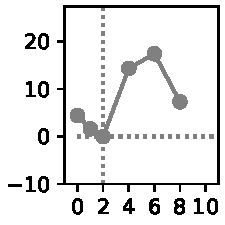
\includegraphics[width=0.14\textwidth]{figures/evaluateCrossValidationResults_Synthetic_Gardelle_NonF.py_SimulateSynthetic_Parameterized_OtherNoiseLevels_Grid_VarySize.py_180_2_2_N40000_STEEPSHIFTED_STEEPPERIODIC.txt_RelativeLF.pdf}%
  };


  % =======================
  % Only 1 Level (Low Noise)
  % =======================
  \node[anchor=center,font=\bfseries] (t1) at (0.45\textwidth, -5.5) {Only 1 Level (Low Noise)};

  % Row 1: first 4 PDFs
  \node (l1a) at (0, -6) {%
    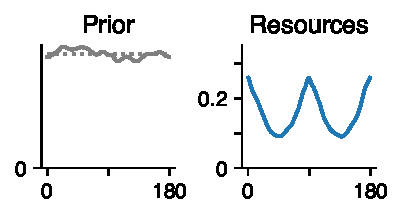
\includegraphics[width=0.3\textwidth]{figures/RunSynthetic_FreePrior_CosineLoss_OnSim_VIZ_OnlyModel_OtherNoiseLevels_WithGroundTruthPrior.py_SimulateSynthetic_Parameterized_OtherNoiseLevels_Grid_VarySize.py_180_2_5_N40000_UNIFORM_STEEPPERIODIC.txt_2_0_10.0_180.pdf}%
  };
  \node (l1b) at (0.3\textwidth, -6) {%
    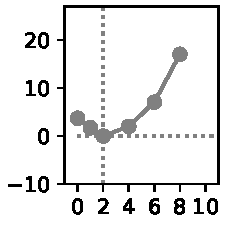
\includegraphics[width=0.14\textwidth]{figures/evaluateCrossValidationResults_Synthetic_Gardelle_NonF.py_SimulateSynthetic_Parameterized_OtherNoiseLevels_Grid_VarySize.py_180_2_5_N40000_UNIFORM_STEEPPERIODIC.txt_RelativeLF.pdf}%
  };
  \node (l1c) at (0.5\textwidth, -6) {%
    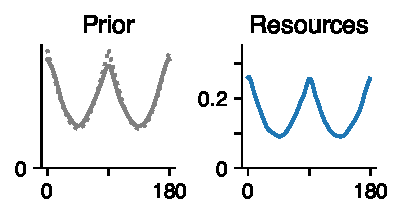
\includegraphics[width=0.3\textwidth]{figures/RunSynthetic_FreePrior_CosineLoss_OnSim_VIZ_OnlyModel_OtherNoiseLevels_WithGroundTruthPrior.py_SimulateSynthetic_Parameterized_OtherNoiseLevels_Grid_VarySize.py_180_2_5_N40000_STEEPPERIODIC_STEEPPERIODIC.txt_2_0_10.0_180.pdf}%
  };
  \node (l1d) at (0.8\textwidth, -6) {%
    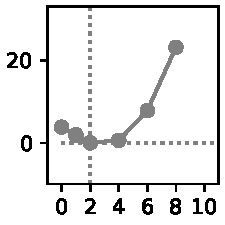
\includegraphics[width=0.14\textwidth]{figures/evaluateCrossValidationResults_Synthetic_Gardelle_NonF.py_SimulateSynthetic_Parameterized_OtherNoiseLevels_Grid_VarySize.py_180_2_5_N40000_STEEPPERIODIC_STEEPPERIODIC.txt_RelativeLF.pdf}%
  };

  % Row 2: next 4 PDFs
  \node (l2a) at (0, -8.5) {%
    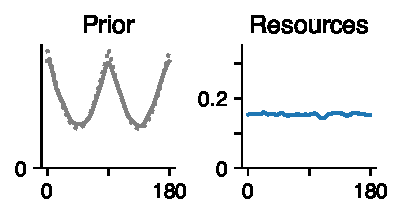
\includegraphics[width=0.3\textwidth]{figures/RunSynthetic_FreePrior_CosineLoss_OnSim_VIZ_OnlyModel_OtherNoiseLevels_WithGroundTruthPrior.py_SimulateSynthetic_Parameterized_OtherNoiseLevels_Grid_VarySize.py_180_2_5_N40000_STEEPPERIODIC_UNIFORM.txt_2_0_10.0_180.pdf}%
  };
  \node (l2b) at (0.3\textwidth, -8.5) {%
    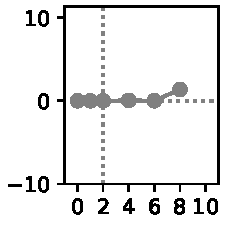
\includegraphics[width=0.14\textwidth]{figures/evaluateCrossValidationResults_Synthetic_Gardelle_NonF.py_SimulateSynthetic_Parameterized_OtherNoiseLevels_Grid_VarySize.py_180_2_5_N40000_STEEPPERIODIC_UNIFORM.txt_RelativeLF.pdf}%
  };
  \node (l2c) at (0.5\textwidth, -8.5) {%
    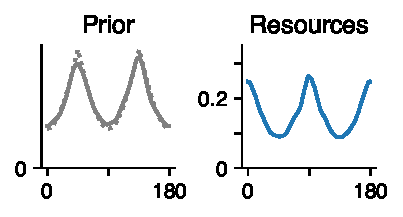
\includegraphics[width=0.3\textwidth]{figures/RunSynthetic_FreePrior_CosineLoss_OnSim_VIZ_OnlyModel_OtherNoiseLevels_WithGroundTruthPrior.py_SimulateSynthetic_Parameterized_OtherNoiseLevels_Grid_VarySize.py_180_2_5_N40000_STEEPSHIFTED_STEEPPERIODIC.txt_2_0_10.0_180.pdf}%
  };
  \node (l2d) at (0.8\textwidth, -8.5) {%
    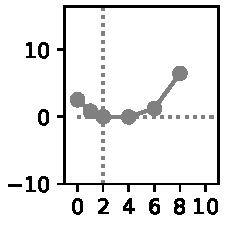
\includegraphics[width=0.14\textwidth]{figures/evaluateCrossValidationResults_Synthetic_Gardelle_NonF.py_SimulateSynthetic_Parameterized_OtherNoiseLevels_Grid_VarySize.py_180_2_5_N40000_STEEPSHIFTED_STEEPPERIODIC.txt_RelativeLF.pdf}%
  };


  % ==============
  % Four Levels
  % ==============
  \node[anchor=center,font=\bfseries] (t1) at (0.45\textwidth, -11.5) {Four Levels};

  % Row 1: first 4 PDFs
  \node (f1a) at (0, -12.0) {%
    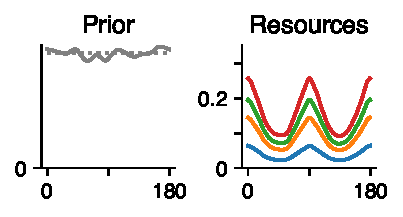
\includegraphics[width=0.3\textwidth]{figures/RunSynthetic_FreePrior_CosineLoss_OnSim_VIZ_OnlyModel_OtherNoiseLevels_WithGroundTruthPrior.py_SimulateSynthetic_Parameterized_OtherNoiseLevels_Grid_VarySize.py_180_2_2345_N40000_UNIFORM_STEEPPERIODIC.txt_2_0_10.0_180.pdf}%
  };
  \node (f1b) at (0.3\textwidth, -12.0) {%
    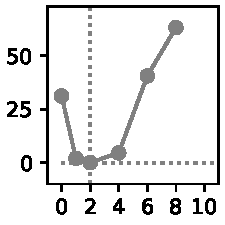
\includegraphics[width=0.14\textwidth]{figures/evaluateCrossValidationResults_Synthetic_Gardelle_NonF.py_SimulateSynthetic_Parameterized_OtherNoiseLevels_Grid_VarySize.py_180_2_2345_N40000_UNIFORM_STEEPPERIODIC.txt_RelativeLF.pdf}%
  };
  \node (f1c) at (0.5\textwidth, -12.0) {%
    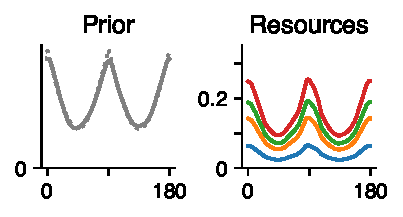
\includegraphics[width=0.3\textwidth]{figures/RunSynthetic_FreePrior_CosineLoss_OnSim_VIZ_OnlyModel_OtherNoiseLevels_WithGroundTruthPrior.py_SimulateSynthetic_Parameterized_OtherNoiseLevels_Grid_VarySize.py_180_2_2345_N40000_STEEPPERIODIC_STEEPPERIODIC.txt_2_0_10.0_180.pdf}%
  };
  \node (f1d) at (0.8\textwidth, -12.0) {%
    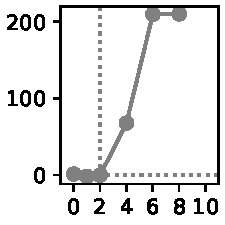
\includegraphics[width=0.14\textwidth]{figures/evaluateCrossValidationResults_Synthetic_Gardelle_NonF.py_SimulateSynthetic_Parameterized_OtherNoiseLevels_Grid_VarySize.py_180_2_2345_N40000_STEEPPERIODIC_STEEPPERIODIC.txt_RelativeLF.pdf}%
  };

  % Row 2: next 4 PDFs
  \node (f2a) at (0, -14.5) {%
    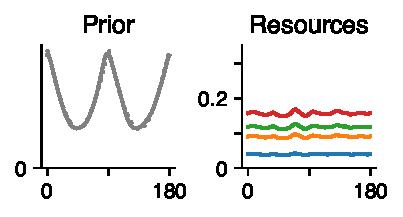
\includegraphics[width=0.3\textwidth]{figures/RunSynthetic_FreePrior_CosineLoss_OnSim_VIZ_OnlyModel_OtherNoiseLevels_WithGroundTruthPrior.py_SimulateSynthetic_Parameterized_OtherNoiseLevels_Grid_VarySize.py_180_2_2345_N40000_STEEPPERIODIC_UNIFORM.txt_2_0_10.0_180.pdf}%
  };
  \node (f2b) at (0.3\textwidth, -14.5) {%
    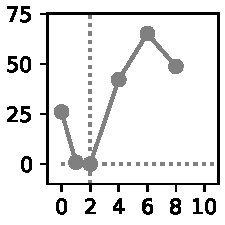
\includegraphics[width=0.14\textwidth]{figures/evaluateCrossValidationResults_Synthetic_Gardelle_NonF.py_SimulateSynthetic_Parameterized_OtherNoiseLevels_Grid_VarySize.py_180_2_2345_N40000_STEEPPERIODIC_UNIFORM.txt_RelativeLF.pdf}%
  };
  \node (f2c) at (0.5\textwidth, -14.5) {%
    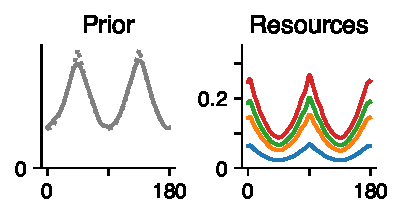
\includegraphics[width=0.3\textwidth]{figures/RunSynthetic_FreePrior_CosineLoss_OnSim_VIZ_OnlyModel_OtherNoiseLevels_WithGroundTruthPrior.py_SimulateSynthetic_Parameterized_OtherNoiseLevels_Grid_VarySize.py_180_2_2345_N40000_STEEPSHIFTED_STEEPPERIODIC.txt_2_0_10.0_180.pdf}%
  };
  \node (f2d) at (0.8\textwidth, -14.5) {%
    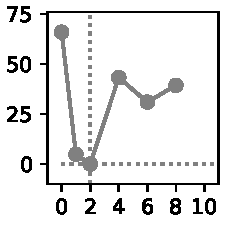
\includegraphics[width=0.14\textwidth]{figures/evaluateCrossValidationResults_Synthetic_Gardelle_NonF.py_SimulateSynthetic_Parameterized_OtherNoiseLevels_Grid_VarySize.py_180_2_2345_N40000_STEEPSHIFTED_STEEPPERIODIC.txt_RelativeLF.pdf}%
  };

\end{tikzpicture}

\caption{Fits at one or four levels of sensory noise, for four combinations of prior (left) and encoding (middle), with ground truth exponent $p=2$. We show both the prior and encoding recovered when fitting at the ground truth exponent ($p=2$), and NLL over exponents (right). Results at 40K trials. At 1 level of sensory noise, NLL does not reliably single out the correct loss function. High noise can lead to a large $\Delta NLL$, but does not reliably distinguish high from low exponents. The shape of the prior is also recovered incorrectly in some cases even when presupposing the correct $p$. Low noise leads to more reliable recovery, but the statistical signal in $\Delta NLL$ can be weak. At four levels of sensory noise, both the prior and the loss function are recovered reliably.}\label{fig:known-loss-unknown-prior}
\begin{comment}
. ./plotSingleNoiseFits.sh
\end{comment}
\end{figure}


\begin{figure}
\centering
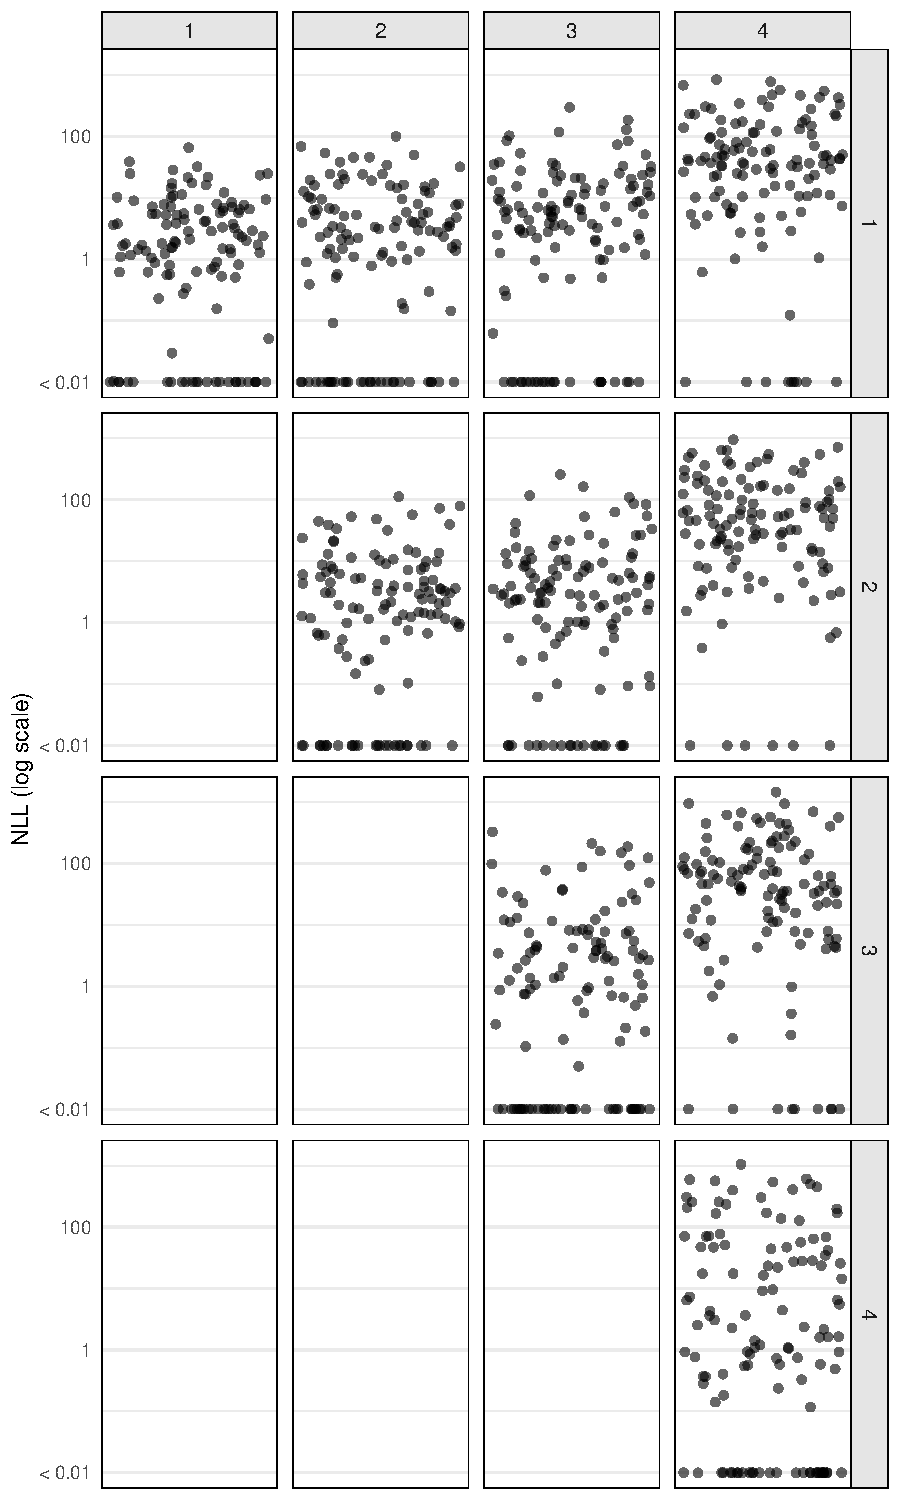
\includegraphics[width=0.6\textwidth]{../code/output/images/sensory_LVL_dotplots.pdf}

\caption{
Subset of the datapoints of Main Paper Figure 5c at N=40,000 trials and one or two noise levels, broken down by the two noise levels (1=smallest noise, 4=largest noise).
Panels on the diagonal correspond to settings with only one noise level.
As we also found in Figure~\ref{fig:known-loss-unknown-prior}, higher noise levels tend to lead to higher $\Delta$ NLL, though, on their own, they often are not sufficient for singling out the ground-truth loss (Figure~\ref{fig:known-loss-unknown-prior}).
Here, we find that across noise magnitudes, combining with a different noise level boosts $\Delta$ NLL (and thus identifiability), and mainly so when combining with a substantially different level (e.g., combining level 1 with level 4).
Intuitively, more distinct noise levels may be more likely to provide complementary evidence about the model; Theorem 3 formalizes this by requiring that the ratio of noise magnitudes be bounded away from 1.
}\label{fig:by-pair-plot}
\end{figure}

Further, see Figure~\ref{fig:known-loss-unknown-prior} for recoverability of these four models at $p=2$, specifically at one or four levels of sensory noise.
Further, see Figure~\ref{fig:by-pair-plot} for results at one or two noise levels, broken down by pairs of noise levels.



\end{document}
